\documentclass[11pt]{article}
\usepackage[utf8]{inputenc}
\usepackage[T1]{fontenc}
\usepackage[spanish]{babel}
\usepackage{graphicx}
\usepackage{float}
\usepackage{amsmath}
\usepackage{booktabs}
\usepackage{listings}
\usepackage{xcolor}
\usepackage[margin=2.5cm]{geometry}

\graphicspath{{graficas/}}

\lstset{
    language=Python,
    basicstyle=\ttfamily\footnotesize,
    keywordstyle=\color{blue},
    commentstyle=\color{gray},
    stringstyle=\color{red!60!black},
    breaklines=true,
    frame=single,
    numbers=left,
    numberstyle=\tiny\color{gray},
    showstringspaces=false,
    literate={á}{{\'a}}1 {é}{{\'e}}1 {í}{{\'i}}1 {ó}{{\'o}}1 {ú}{{\'u}}1 {ñ}{{\~n}}1
}

\title{Proyecto Final de An\'alisis Num\'erico\\
\large Interpolaci\'on de la poblaci\'on de Ucrania (1994--2023)\\
con Lagrange y Trazadores C\'ubicos Naturales}
\author{Pau V\\
Pontificia Universidad Javeriana\\
Facultad de Ciencias, Departamento de Matem\'aticas\\
An\'alisis Num\'erico}
\date{Noviembre 2026}

\begin{document}
\maketitle

\section{Introducci\'on}

El objetivo del proyecto es comparar el desempe\~no de los polinomios de Lagrange
y de los trazadores c\'ubicos para interpolar un conjunto numeroso de datos. Para
ello se aproxima la poblaci\'on de Ucrania (el pa\'is asignado) entre 1994 y 2023
a partir de datos discretos. El conjunto de datos tiene 30 registros anuales: 25
sirven como nodos de interpolaci\'on y 5 (los resaltados en el Excel) se
reservan como datos de prueba. Los 5 a\~nos de prueba son 1994, 2002, 2009, 2017
y 2023.

Se comparan dos m\'etodos:
\begin{itemize}
    \item el polinomio interpolador de \textbf{Lagrange} de grado 24, y
    \item el \textbf{trazador c\'ubico natural}, que usa un polinomio c\'ubico por tramo.
\end{itemize}
La calidad de cada m\'etodo se mide con el error relativo
$E_r = \dfrac{|y_{\text{exacto}} - y_{\text{aprox}}|}{|y_{\text{exacto}}|}$.

\section{Implementaci\'on de los Algoritmos}

Se eligi\'o \textbf{Python 3} por su sintaxis clara y por la facilidad para leer
datos estructurados y generar gr\'aficas. El proyecto es modular: cada algoritmo
vive en su propio archivo y se puede ejecutar de forma independiente.

\subsection{Estructura del programa}
\begin{itemize}
    \item \texttt{datos.py}: lee el archivo Excel y separa nodos y datos de prueba.
    \item \texttt{Lagrange/lagrange.py}: polinomio interpolador de Lagrange.
    \item \texttt{Trazadores/trazadores.py}: trazador c\'ubico natural (algoritmo de Thomas).
    \item \texttt{graficas.py}: genera las curvas y los diagramas de error en formato PNG.
\end{itemize}

\subsection{Captura y organizaci\'on de datos (\texttt{datos.py})}
El Excel tiene 30 registros (1994--2023). Las 25 filas sin color de relleno son
los nodos y las 5 filas con relleno s\'olido son los datos de prueba.

\begin{lstlisting}
def cargar_datos(ruta=EXCEL):
    ws = openpyxl.load_workbook(ruta).active
    x, y, xr, yr = [], [], [], []
    for fila in range(2, ws.max_row + 1):
        anio, pob = ws.cell(fila, 2), ws.cell(fila, 3)
        if anio.value is None or pob.value is None:
            continue
        # Celdas con color -> datos resaltados a aproximar
        if anio.fill.fill_type == "solid":
            xr.append(anio.value)
            yr.append(pob.value)
        else:  # Celdas sin color -> nodos para interpolar
            x.append(anio.value)
            y.append(pob.value)
    return x, y, xr, yr
\end{lstlisting}

\subsection{Algoritmo 1: Polinomio de Lagrange (\texttt{lagrange.py})}
Dados $n=25$ nodos $(x_k, y_k)$, el polinomio interpolador de grado $n-1=24$ es
\[
L_k(x) = \prod_{j \neq k} \frac{x - x_j}{x_k - x_j}, \qquad
P(x) = \sum_{k=0}^{n-1} y_k\, L_k(x).
\]

\begin{lstlisting}
def base_lagrange(x, nodos, k):
    """L_k(x) = prod_{j != k} (x - x_j) / (x_k - x_j)"""
    L = 1.0
    for j, xj in enumerate(nodos):
        if j != k:
            L *= (x - xj) / (nodos[k] - xj)
    return L

def lagrange(x, nodos, valores):
    """P(x) = sum_k y_k * L_k(x), con todos los nodos dados."""
    return sum(valores[k] * base_lagrange(x, nodos, k)
               for k in range(len(nodos)))

def error_relativo(exacto, aprox):
    return abs(exacto - aprox) / abs(exacto)
\end{lstlisting}

\subsection{Algoritmo 2: Trazador c\'ubico natural (\texttt{trazadores.py})}
Los polinomios de grado alto oscilan mucho. Para evitarlo se implement\'o el
\textbf{Algoritmo 3.4 de Burden \& Faires}. En cada tramo $[x_j, x_{j+1}]$ se usa
\[
S_j(x) = a_j + b_j (x - x_j) + c_j (x - x_j)^2 + d_j (x - x_j)^3,
\]
con condiciones de frontera naturales $S''(x_0) = S''(x_n) = 0$. Los coeficientes
$c_j$ salen de un sistema tridiagonal, que se resuelve en $O(n)$ con el
algoritmo de Thomas (factorizaci\'on de Crout).

\begin{lstlisting}
def construir_trazador_cubico_natural(nodos, valores):
    puntos = sorted(zip(nodos, valores))
    x = [float(p[0]) for p in puntos]
    a = [float(p[1]) for p in puntos]
    n = len(x) - 1

    # Anchos de subintervalos h_i
    h = [x[i + 1] - x[i] for i in range(n)]

    # Vector alpha del sistema tridiagonal
    alpha = [0.0] * (n + 1)
    for i in range(1, n):
        alpha[i] = (3.0 / h[i]) * (a[i + 1] - a[i]) \
                 - (3.0 / h[i - 1]) * (a[i] - a[i - 1])

    # Algoritmo de Thomas (Crout)
    l = [1.0] + [0.0] * n
    mu = [0.0] * (n + 1)
    z = [0.0] * (n + 1)
    for i in range(1, n):
        l[i] = 2.0 * (x[i + 1] - x[i - 1]) - h[i - 1] * mu[i - 1]
        mu[i] = h[i] / l[i]
        z[i] = (alpha[i] - h[i - 1] * z[i - 1]) / l[i]

    # Fronteras naturales: c_0 = 0 y c_n = 0
    l[n], z[n] = 1.0, 0.0
    c = [0.0] * (n + 1)
    b = [0.0] * n
    d = [0.0] * n

    # Sustitucion hacia atras
    for j in range(n - 1, -1, -1):
        c[j] = z[j] - mu[j] * c[j + 1]
        b[j] = (a[j + 1] - a[j]) / h[j] \
             - h[j] * (c[j + 1] + 2.0 * c[j]) / 3.0
        d[j] = (c[j + 1] - c[j]) / (3.0 * h[j])

    return x, a[:n], b, c[:n], d
\end{lstlisting}

\subsection{Tabla de variables principales}
\begin{table}[H]
\centering
\small
\begin{tabular}{|l|l|p{7.5cm}|}
\hline
\textbf{Variable} & \textbf{Tipo} & \textbf{Descripci\'on} \\ \hline
\texttt{nodos} / \texttt{x} & \texttt{list[float]} & A\~nos conocidos $x_i$ usados como nodos ($n=25$). \\ \hline
\texttt{valores} / \texttt{a} & \texttt{list[float]} & Poblaci\'on conocida $y_i = a_i$ en los nodos. \\ \hline
\texttt{resaltados} & \texttt{list[int]} & A\~nos de prueba (5 datos) para validar los m\'etodos. \\ \hline
\texttt{h} & \texttt{list[float]} & Distancias entre nodos consecutivos $h_i = x_{i+1} - x_i$. \\ \hline
\texttt{alpha} & \texttt{list[float]} & Lado derecho del sistema tridiagonal. \\ \hline
\texttt{l, mu, z} & \texttt{list[float]} & Vectores auxiliares de la factorizaci\'on de Crout. \\ \hline
\texttt{b, c, d} & \texttt{list[float]} & Coeficientes lineal, cuadr\'atico y c\'ubico de cada tramo. \\ \hline
\end{tabular}
\caption{Variables principales del sistema de interpolaci\'on.}
\end{table}

\subsection{Diagramas de flujo}
Los flujos l\'ogicos de los m\'odulos se modelaron en Mermaid y se exportaron a
PDF para mantener la nitidez en la impresi\'on.

\begin{figure}[H]
    \centering
    \includegraphics[width=0.45\textwidth]{flujo_datos.pdf}
    \caption{Flujo de datos de \texttt{cargar\_datos}.}
\end{figure}

\begin{figure}[H]
    \centering
    \includegraphics[width=0.45\textwidth]{algoritmo_lagrange.pdf}
    \caption{Flujo del algoritmo de Lagrange.}
\end{figure}

\begin{figure}[H]
    \centering
    \includegraphics[width=0.45\textwidth]{algoritmo_trazadores.pdf}
    \caption{Flujo del trazador c\'ubico natural.}
\end{figure}

\section{Resultados}

Se evaluaron ambos m\'etodos en los 5 a\~nos de prueba, usando solo los 25 nodos.

\begin{table}[H]
\centering
\small
\begin{tabular}{rrrr}
\toprule
A\~no & Valor exacto & Lagrange & Error relativo \\
\midrule
1994 & 52\,076\,000 & $-21\,736\,816\,040{,}49$ & $418{,}4056386913$ \\
2002 & 48\,677\,280 & 48\,695\,338{,}85 & $0{,}0003709914$ \\
2009 & 46\,623\,731 & 46\,608\,582{,}57 & $0{,}0003249082$ \\
2017 & 45\,436\,037 & 45\,753\,319{,}55 & $0{,}0069830595$ \\
2023 & 37\,732\,833 & $-33\,412\,276\,260{,}07$ & $886{,}4960946100$ \\
\bottomrule
\end{tabular}
\caption{Interpolaci\'on de Lagrange (grado 24).}
\end{table}

\begin{table}[H]
\centering
\small
\begin{tabular}{rrrr}
\toprule
A\~no & Valor exacto & Trazador c\'ubico & Error relativo \\
\midrule
1994 & 52\,076\,000 & 52\,104\,959{,}00 & $0{,}0005560911$ \\
2002 & 48\,677\,280 & 48\,683\,629{,}82 & $0{,}0001304474$ \\
2009 & 46\,623\,731 & 46\,618\,926{,}17 & $0{,}0001030555$ \\
2017 & 45\,436\,037 & 45\,420\,397{,}18 & $0{,}0003442162$ \\
2023 & 37\,732\,833 & 37\,798\,894{,}00 & $0{,}0017507564$ \\
\bottomrule
\end{tabular}
\caption{Trazador c\'ubico natural (24 tramos).}
\end{table}

\begin{figure}[H]
    \centering
    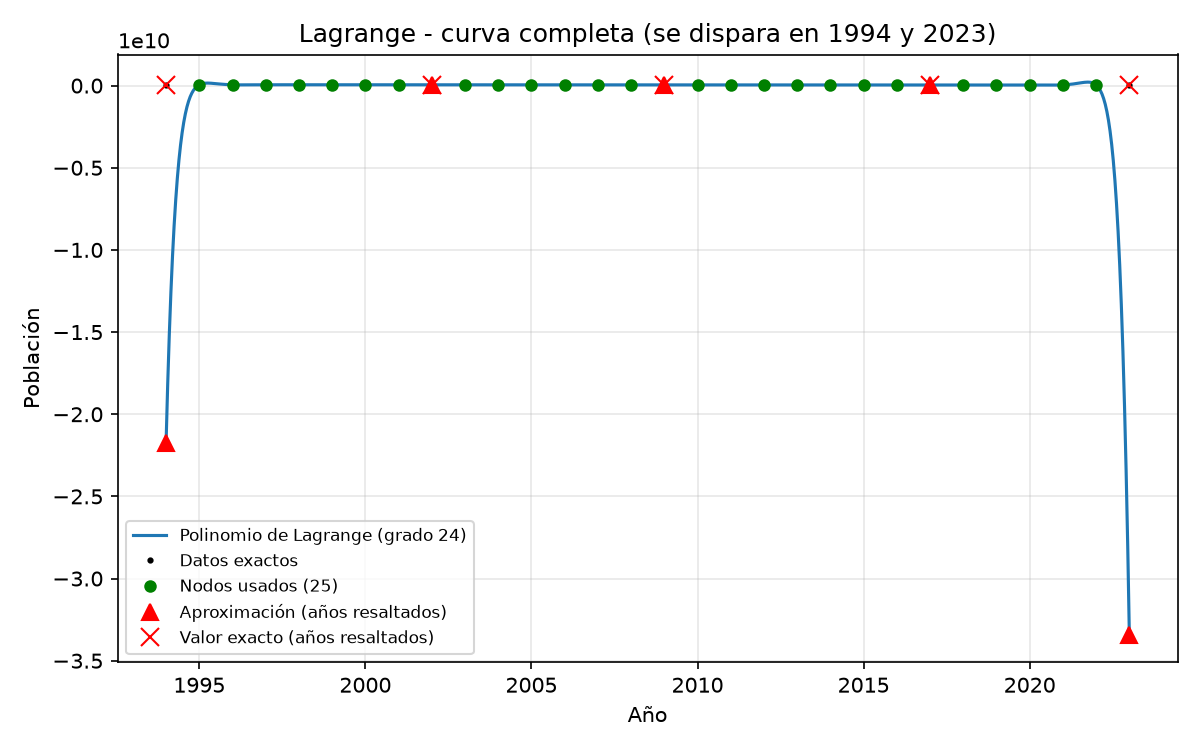
\includegraphics[width=0.9\linewidth]{lagrange_curva_completa.png}
    \caption{Polinomio de Lagrange en todo el rango 1994--2023: se dispara en los extremos.}
\end{figure}

\begin{figure}[H]
    \centering
    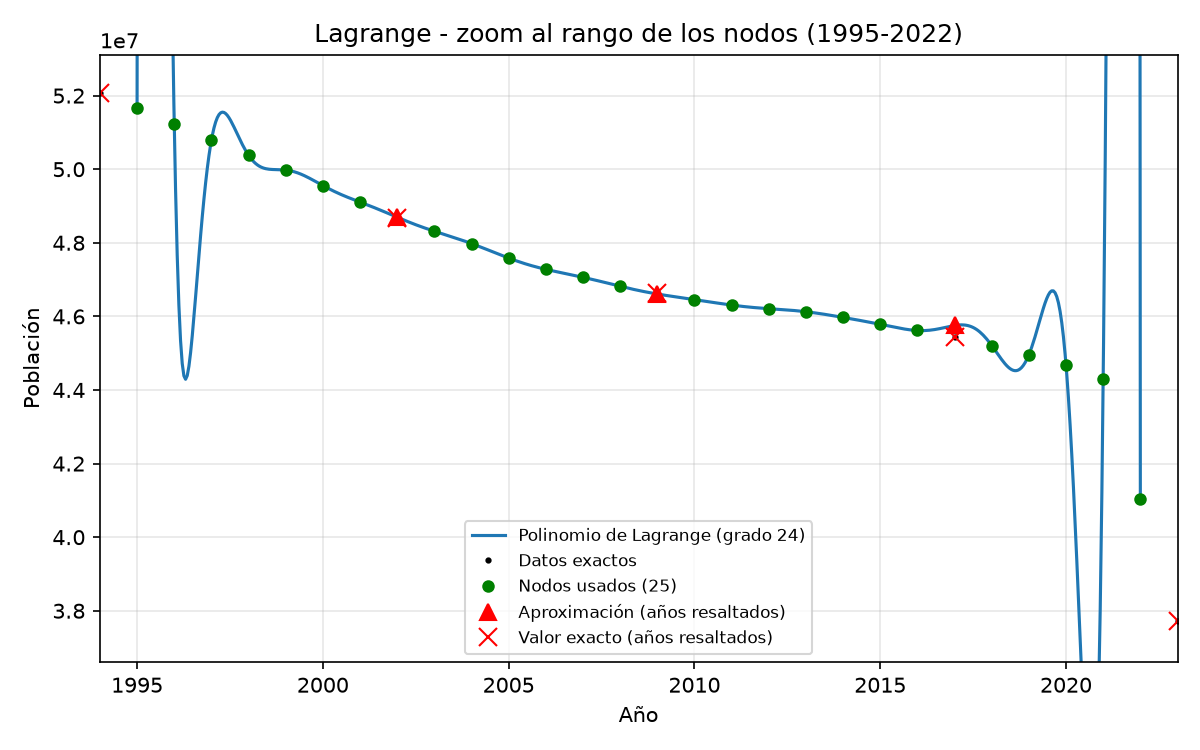
\includegraphics[width=0.9\linewidth]{lagrange_zoom.png}
    \caption{Lagrange ampliado al rango de los nodos (1995--2022).}
\end{figure}

\begin{figure}[H]
    \centering
    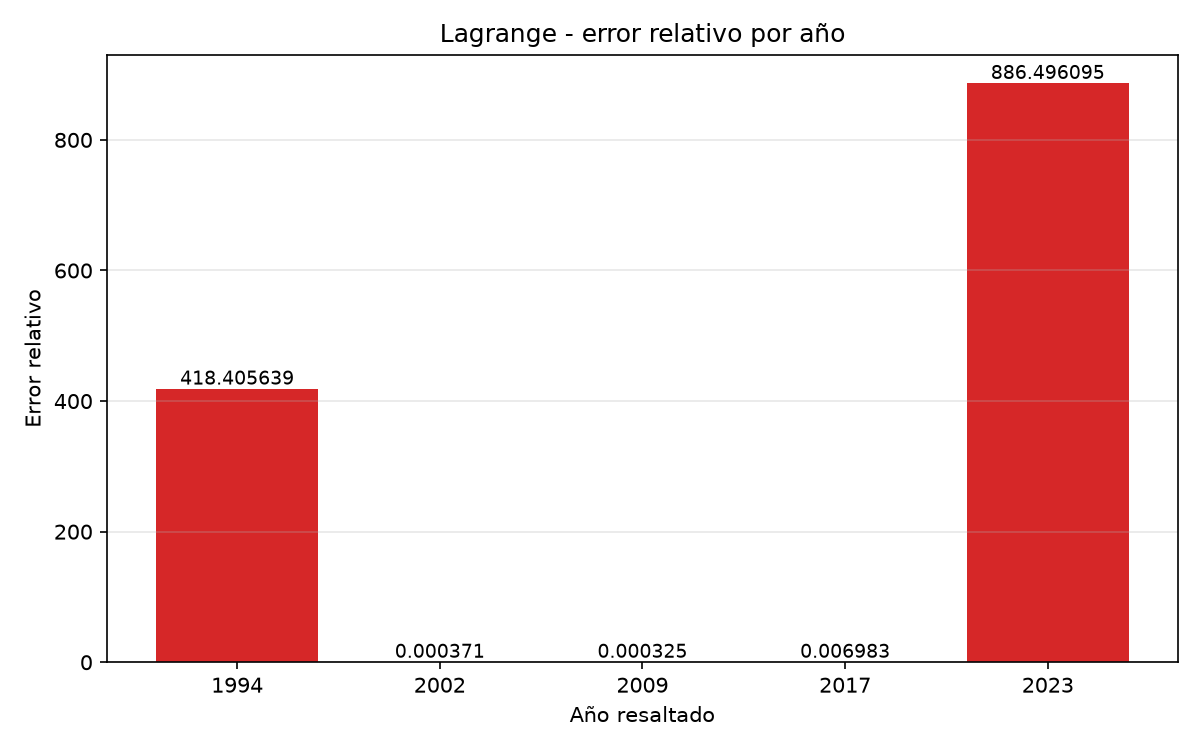
\includegraphics[width=0.9\linewidth]{lagrange_errores.png}
    \caption{Error relativo de Lagrange por a\~no de prueba.}
\end{figure}

\begin{figure}[H]
    \centering
    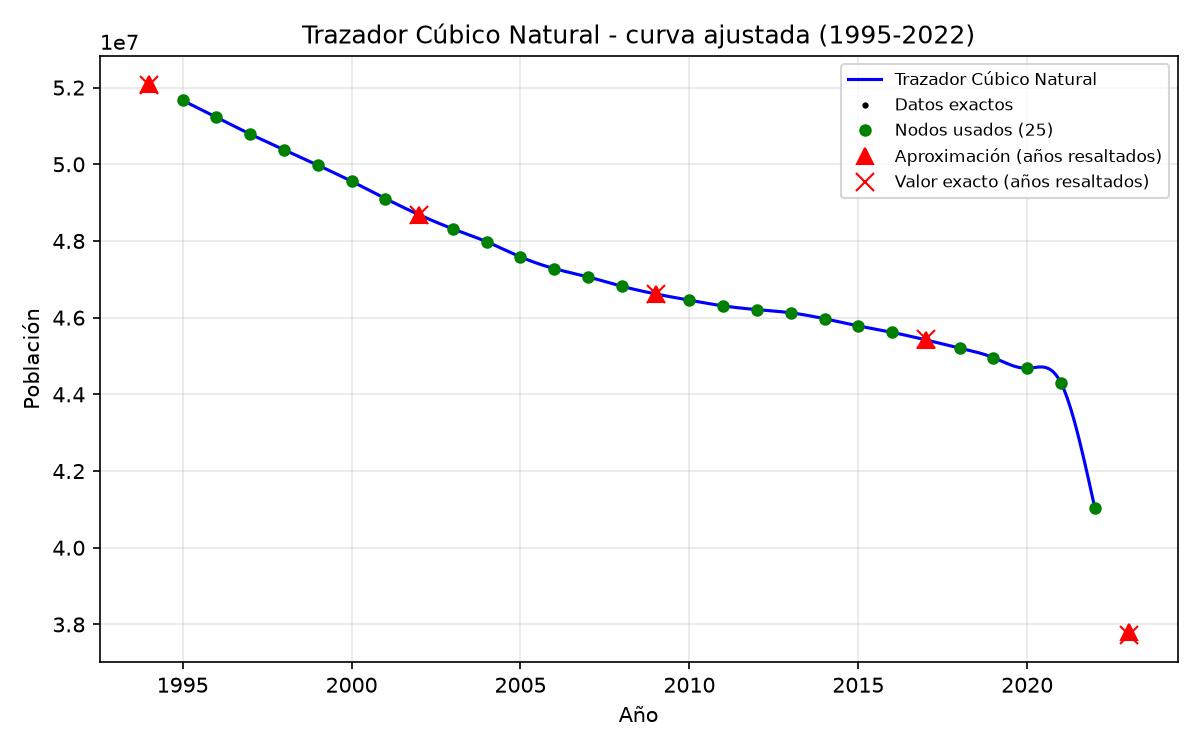
\includegraphics[width=0.9\linewidth]{trazador_curva.png}
    \caption{Trazador c\'ubico natural ajustado a los nodos.}
\end{figure}

\begin{figure}[H]
    \centering
    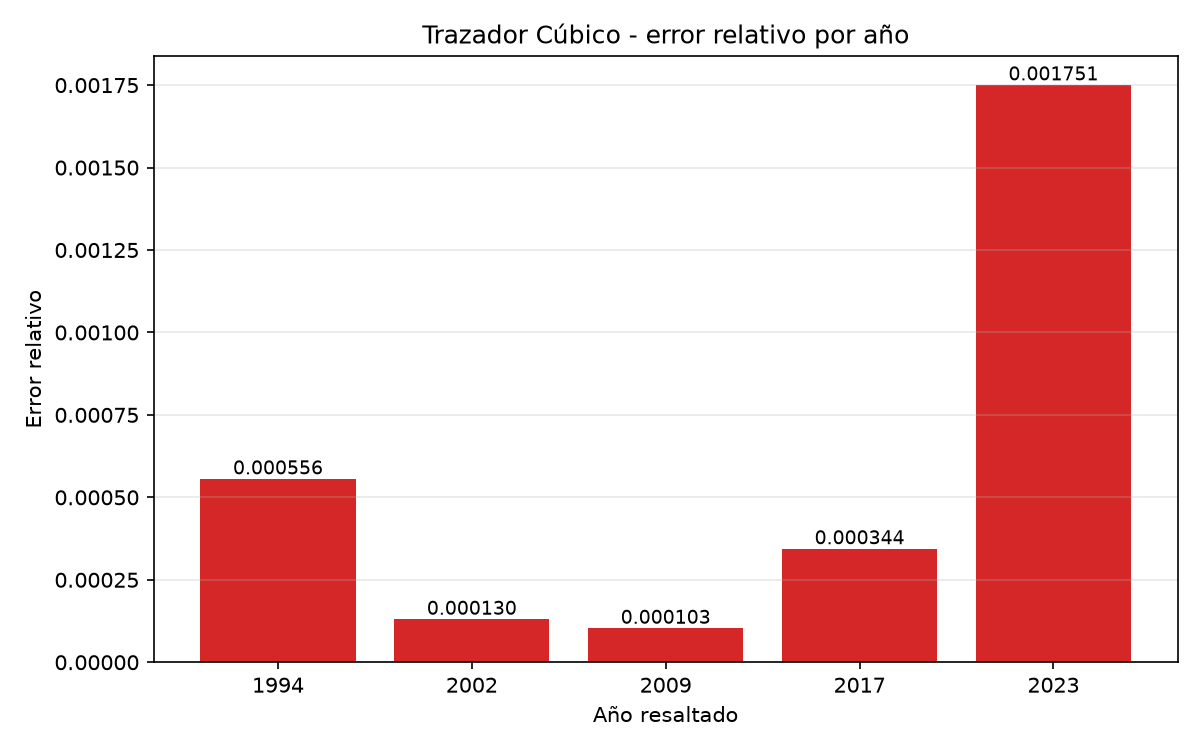
\includegraphics[width=0.9\linewidth]{trazador_errores.png}
    \caption{Error relativo del trazador c\'ubico por a\~no de prueba.}
\end{figure}

\subsection{Comparaci\'on entre ambos m\'etodos}

\begin{table}[H]
\centering
\small
\begin{tabular}{rrrr}
\toprule
A\~no & Valor exacto & Error rel. Lagrange & Error rel. trazador \\
\midrule
1994 & 52\,076\,000 & $418{,}4056$ & $0{,}000556$ \\
2002 & 48\,677\,280 & $0{,}000371$ & $0{,}000130$ \\
2009 & 46\,623\,731 & $0{,}000325$ & $0{,}000103$ \\
2017 & 45\,436\,037 & $0{,}006983$ & $0{,}000344$ \\
2023 & 37\,732\,833 & $886{,}4961$ & $0{,}001751$ \\
\bottomrule
\end{tabular}
\caption{Comparaci\'on del error relativo de ambos m\'etodos en los a\~nos resaltados.}
\end{table}

\begin{figure}[H]
    \centering
    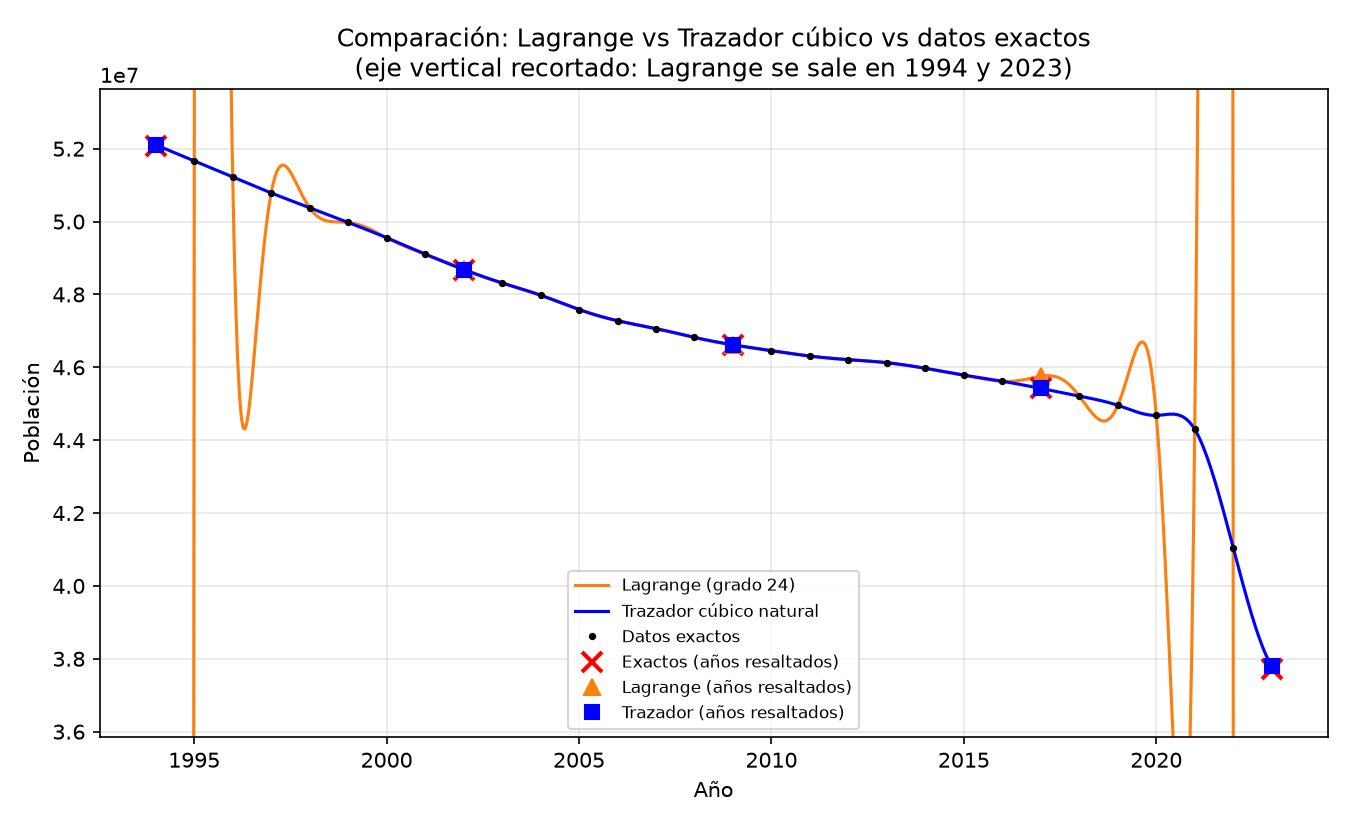
\includegraphics[width=\linewidth]{comparacion_curvas.png}
    \caption{Lagrange, trazador c\'ubico y valores exactos en una sola gr\'afica. El eje vertical
    est\'a recortado para poder ver los datos; Lagrange se sale de la gr\'afica en 1994 y 2023.}
\end{figure}

\begin{figure}[H]
    \centering
    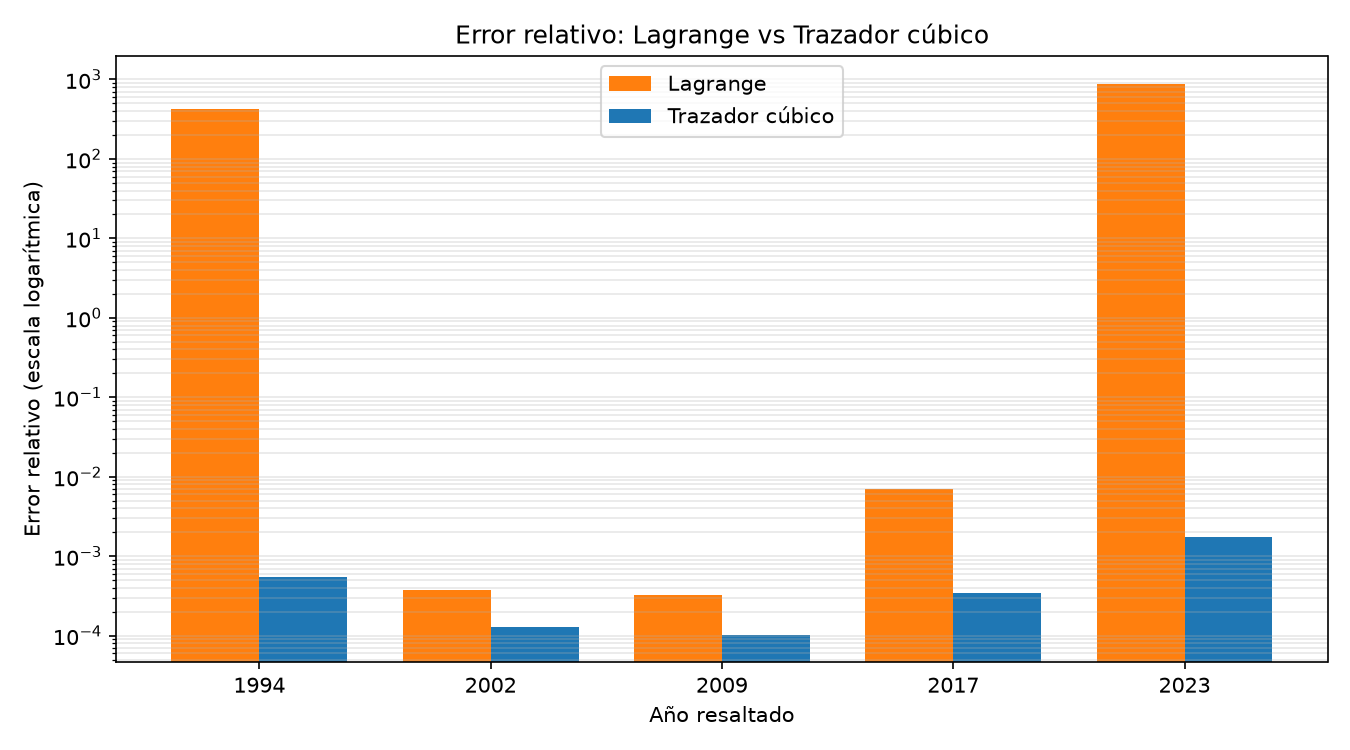
\includegraphics[width=0.9\linewidth]{comparacion_errores.png}
    \caption{Error relativo de ambos m\'etodos en escala logar\'itmica.}
\end{figure}

\section{An\'alisis de resultados}

\begin{itemize}
    \item \textbf{Extrapolaci\'on en 1994 y 2023.} Estos dos a\~nos quedan fuera del
    rango de los nodos (1995--2022), as\'i que ah\'i se \emph{extrapola}. Lagrange
    falla por completo: predice poblaciones negativas del orden de $10^{10}$, con
    errores relativos de 418 y 886 (m\'as de $4\times10^4\,\%$). Es el fen\'omeno
    de Runge: un polinomio de grado 24 oscila con fuerza fuera de los nodos.
    \item \textbf{Interpolaci\'on en 2002, 2009 y 2017.} Dentro del rango, Lagrange
    s\'i aproxima bien, con errores entre $3\times10^{-4}$ y $7\times10^{-3}$. Aun
    as\'i, en 2017 su error ($0{,}70\,\%$) es unas 20 veces mayor que el del
    trazador ($0{,}034\,\%$).
    \item \textbf{Trazador c\'ubico.} Su error m\'aximo es $0{,}175\,\%$ (2023) y
    en los dem\'as a\~nos est\'a por debajo de $0{,}06\,\%$. Al ser polinomios de
    grado 3 por tramo, no oscila y se mantiene cerca de la tendencia de los datos
    incluso al extrapolar.
\end{itemize}

\subsection{\'Por qu\'e se produjeron estas diferencias}
\begin{itemize}
    \item \textbf{Naturaleza global frente a local.} El polinomio de Lagrange es
    \'unico y global: cada nodo influye en toda la curva, y cualquier peque\~na
    irregularidad de los datos se propaga a todo el intervalo. El trazador es
    local: cada tramo depende sobre todo de los nodos vecinos, por lo que un
    error no se esparce.
    \item \textbf{Fen\'omeno de Runge.} Con 25 nodos casi equiespaciados, el
    polinomio de grado 24 oscila en los bordes del intervalo. En la gr\'afica
    se ve que Lagrange ya oscila antes de 1997 y despu\'es de 2019, aun dentro del
    rango de los nodos. Fuera de \'el (1994 y 2023) la oscilaci\'on crece de forma
    explosiva, porque el polinomio es de grado alto.
    \item \textbf{Cambio de tendencia.} La poblaci\'on cae de forma abrupta
    despu\'es de 2021. Un polinomio de grado 24 no logra seguir ese cambio sin
    oscilar, mientras que los tramos c\'ubicos se adaptan a la curvatura local.
    \item \textbf{Condiciones de frontera.} El trazador natural impone $S''=0$ en
    los extremos, lo que limita la curvatura y evita que la curva se dispare
    cuando se extrapola un solo a\~no.
    \item \textbf{Condicionamiento num\'erico.} Los productos de las bases de
    Lagrange mezclan t\'erminos muy grandes y muy peque\~nos y producen
    cancelaci\'on. El sistema tridiagonal del trazador es diagonalmente
    dominante y est\'a bien condicionado.
\end{itemize}

\section{Conclusiones}

\begin{enumerate}
    \item El trazador c\'ubico natural fue m\'as preciso que Lagrange en los 5
    a\~nos de prueba, y la diferencia es enorme en los extremos.
    \item Lagrange con 25 nodos (grado 24) es num\'ericamente inestable cerca de
    los bordes del intervalo. Solo es confiable en el interior del rango de nodos.
    \item Para extrapolar un solo a\~no fuera de los datos, el trazador tambi\'en
    es mucho m\'as razonable (error de $0{,}06\,\%$ en 1994 y $0{,}18\,\%$ en 2023),
    aunque conviene tomar con cautela cualquier extrapolaci\'on.
    \item Para series demogr\'aficas largas es preferible usar trazadores o
    polinomios de grado bajo por tramos, y no un \'unico polinomio de grado alto.
    \item Adem\'as, el algoritmo de Thomas resuelve el sistema tridiagonal en
    $O(n)$, mientras que evaluar Lagrange cuesta $O(n^2)$ por punto.
\end{enumerate}

\end{document}
